\chapter{Prototype}

\begin{figure}[H]
\centering
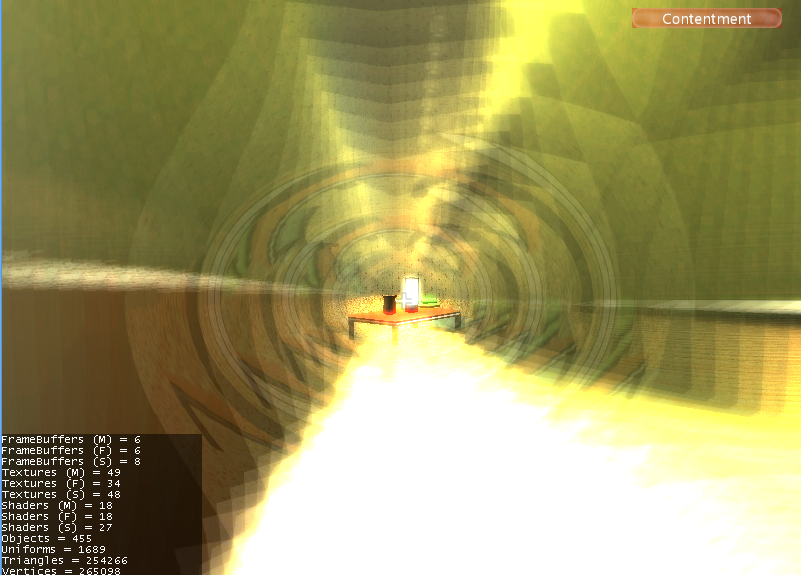
\includegraphics[width=90mm]{images/prototype/overload_livingroom.png}
\caption{Sensory overload in kitchen}
\label{old_house}
\end{figure}

\begin{figure}[H]
\centering
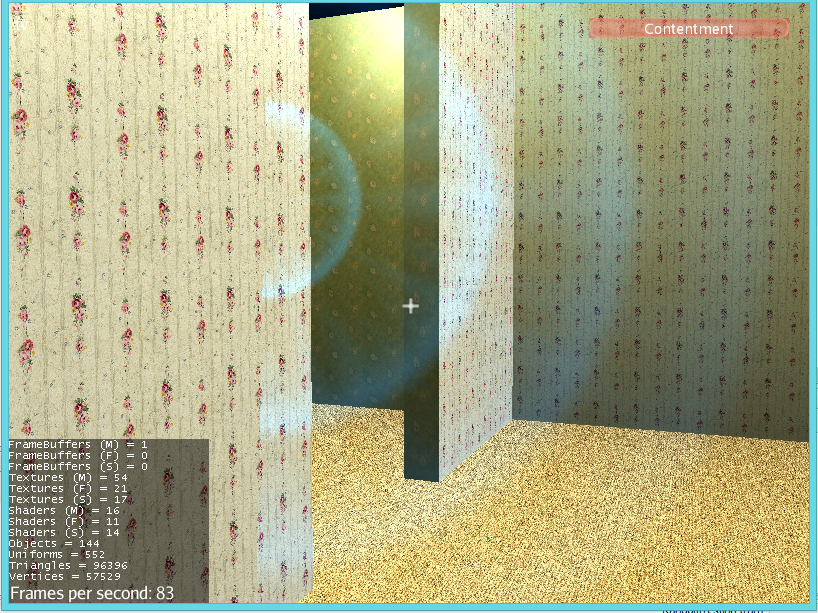
\includegraphics[width=90mm]{images/prototype/visualsounds.png}
\caption{Visual sounds representation}
\label{old_house}
\end{figure}

\chapter{Formative}
\begin{figure}[H]
\centering
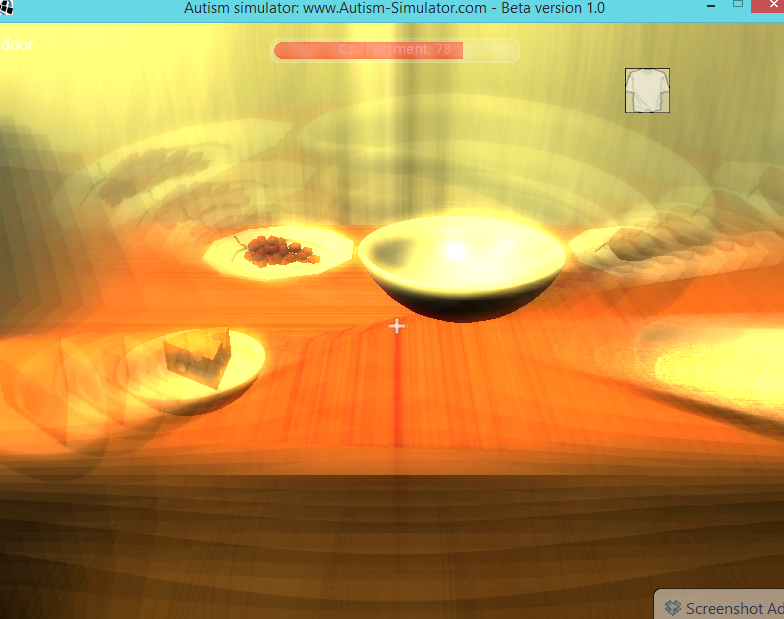
\includegraphics[width=90mm]{images/implementationfirst/gameimages/breakfast_overload.png}
\caption{Sensory overload caused by fluorescent lights in kitchen}
\label{old_house}
\end{figure}

\begin{figure}[H]
\centering
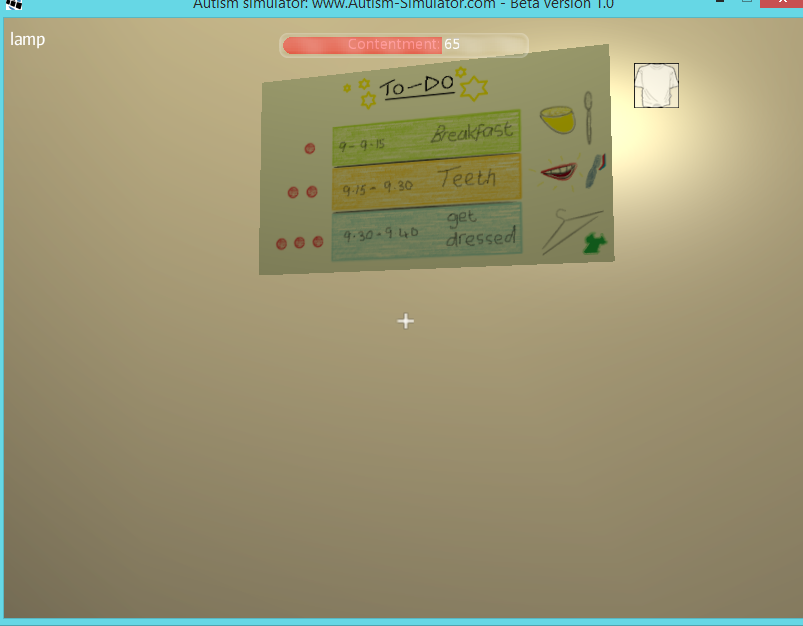
\includegraphics[width=90mm]{images/implementationfirst/gameimages/morningroutine.png}
\caption{Morning routine added to the wall after participant 2 feedback}
\label{old_house}
\end{figure}

\chapter{Participatory design materials}
\label{appendix_partdesign}

\section{LAER Lab}
\begin{figure}[H]
\centering
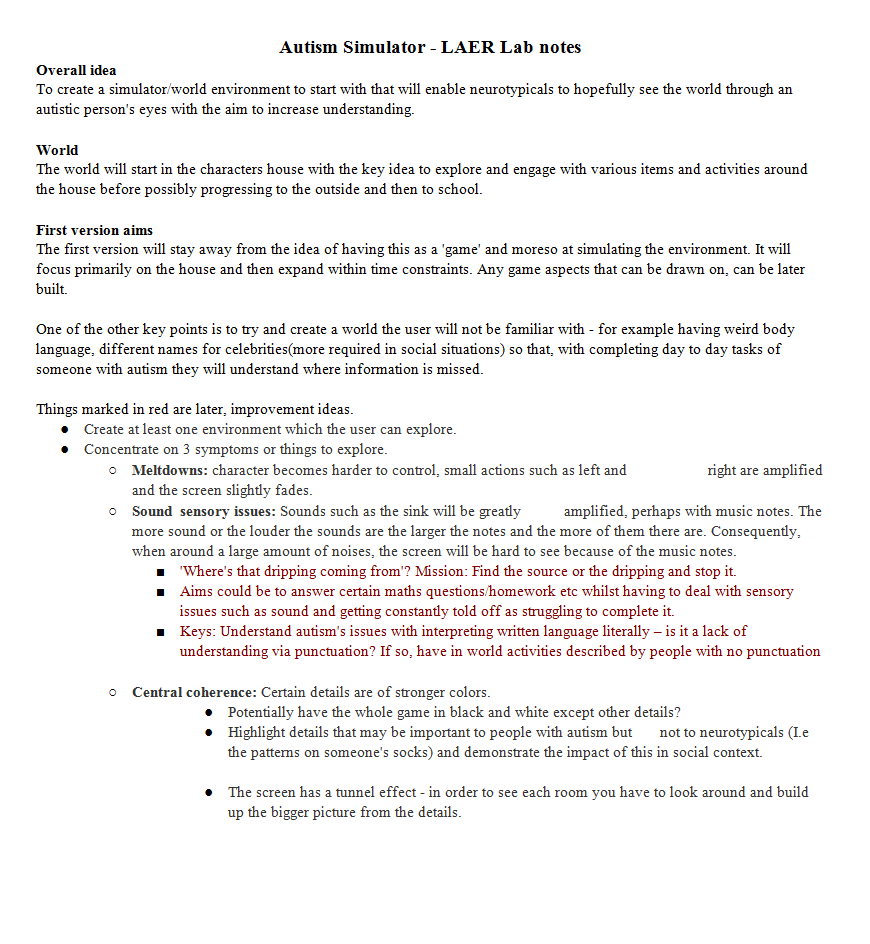
\includegraphics[scale=0.7]{images/appendix/partdesign_laernotesa.png}
\caption{Page 1 of LAER lab notes}
\end{figure}

\begin{figure}[H]
\centering
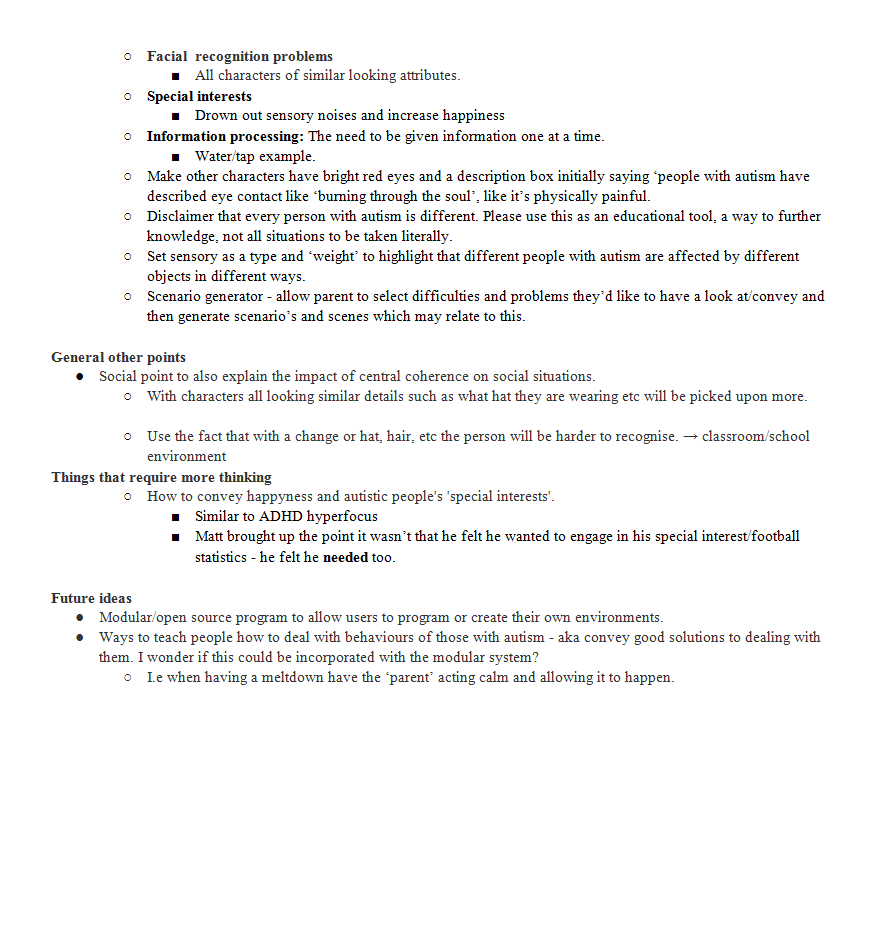
\includegraphics[scale=0.7]{images/appendix/partdesign_laernotesb.png}
\caption{Page 2 of LAER lab notes}
\end{figure}

\section{Interviews}
\subsection{Teacher: Candidate 2}
A: Do you feel this could be a useful tool?\\
T: I think so, definitely. We say every day it would be great to step into their world for even just five minutes. It would be great to have something like that, even if to get just a slight view of what they must be seeing or feeling.\\
A: Hardest skill or aspect required to teach new staff?\\
T: Language and communication and information processing delay. A lot of staff have verbal diarrhea and we have to keep reminding them to give black and white information or questions. Also the delayed processing of information where staff keep repeatedly asking questions without giving them time to think. It’s taking a step back that people need to learn to do and I think if they could just jump into their world for 5 minutes it would greatly aid this”\\
A: What are the consequences of that? Could that lead to a meltdown or...?\\
T: It can do. That or it just leads them to being very unresponsive, you’ll ask them to do something and they just wont.\\
A: Hardest aspect of being in a classroom environment?\\
T: That some of the triggers can send a wave of problems around the classroom. For example if one child is affected by touch and screams...which then affects someone who is very sensitive to sound.\\

\subsection{Candidate 3: Person with autism}
C3: School was very difficult and I could never understand why friendships broke down...except the obvious that I didn’t like people looking at me. \\
A: How did it make you feel when people looked at you?\\
C3: Physically uncomfortable, as if their eyes were burning through me.\\
A: If you couldn’t verbalise your difficulties, how did it make you feel?\\
C3: Awful...even now I can feel the feeling that I can’t put a word too. I was permanently in a very heightened state of anxiety. I always had a bad stomach and skin conditions. It would start on a sunday with the dreading of school on the monday and it kind of went on. \\
A: As a child what would you wish your parents would have done differently or to have helped you as a child?\\
C3: One of them would be finding a different way to communicate.\\
S(random person entering): One random question, could you ever feel storms before they came? Like a change in the atmosphere, you could basically smell it. It’s weird to explain.\\
C3: Yes, definately. I’d feed anxious before it happened and wouldn’t quite know why, until later when the storm came and I finally did.\\

\chapter{Summative}
\label{sec:appendix_summative}

\section{Summative materials}
\label{sec:summative_materials}
\begin{figure}[H]
\centering
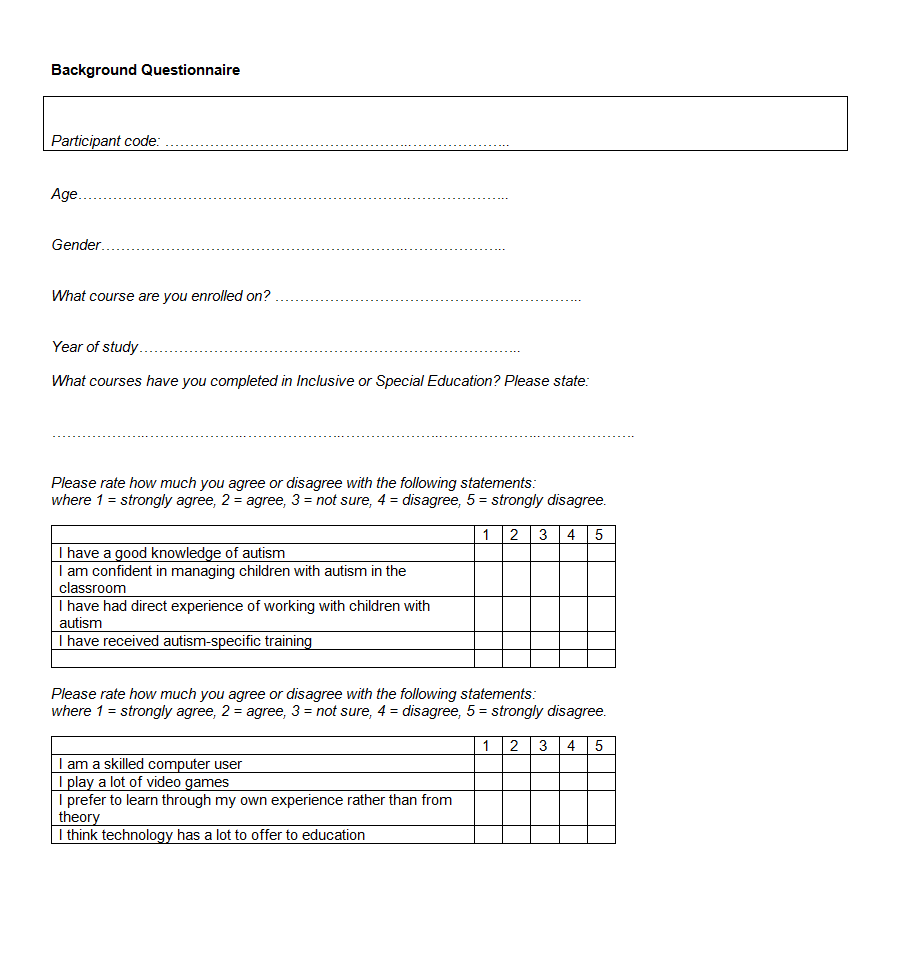
\includegraphics[scale=0.7]{images/appendix/background_q.png}
\caption{Background questionnaire}
\label{sum_background}
\end{figure}

\begin{figure}[H]
\centering
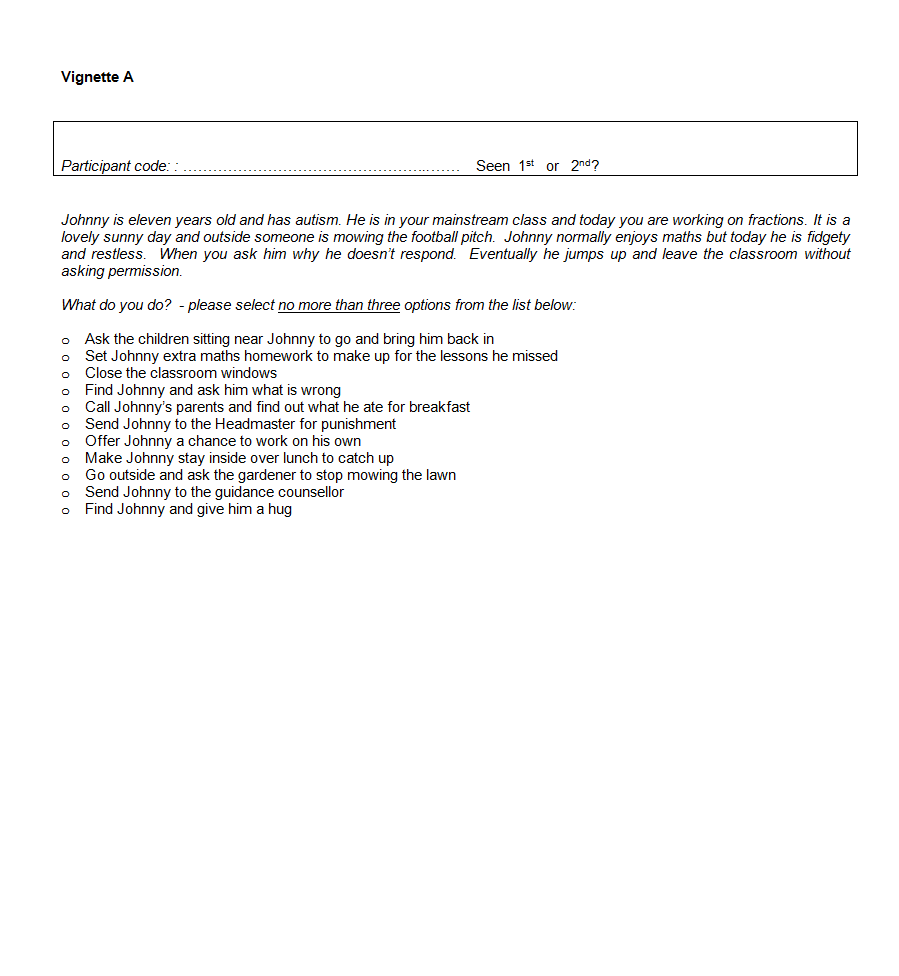
\includegraphics[scale=0.7]{images/appendix/summative_va.png}
\caption{Vignette A}
\end{figure}

\begin{figure}[H]
\centering
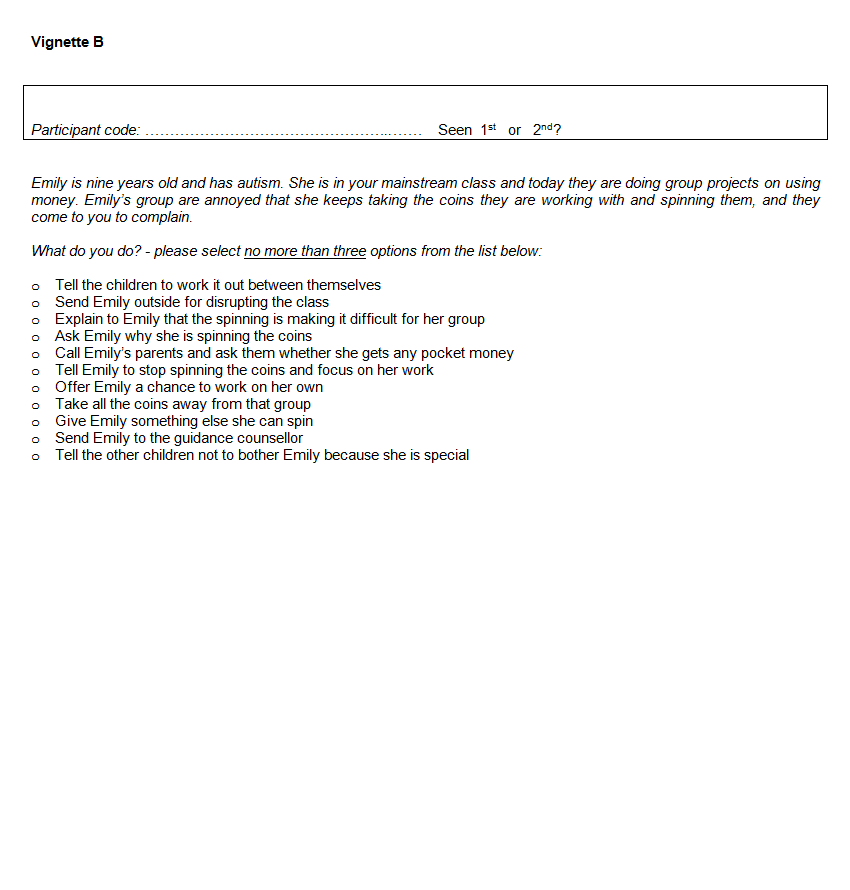
\includegraphics[scale=0.7]{images/appendix/summative_vb.png}
\caption{Vignette B}
\end{figure}

\begin{figure}[H]
\centering
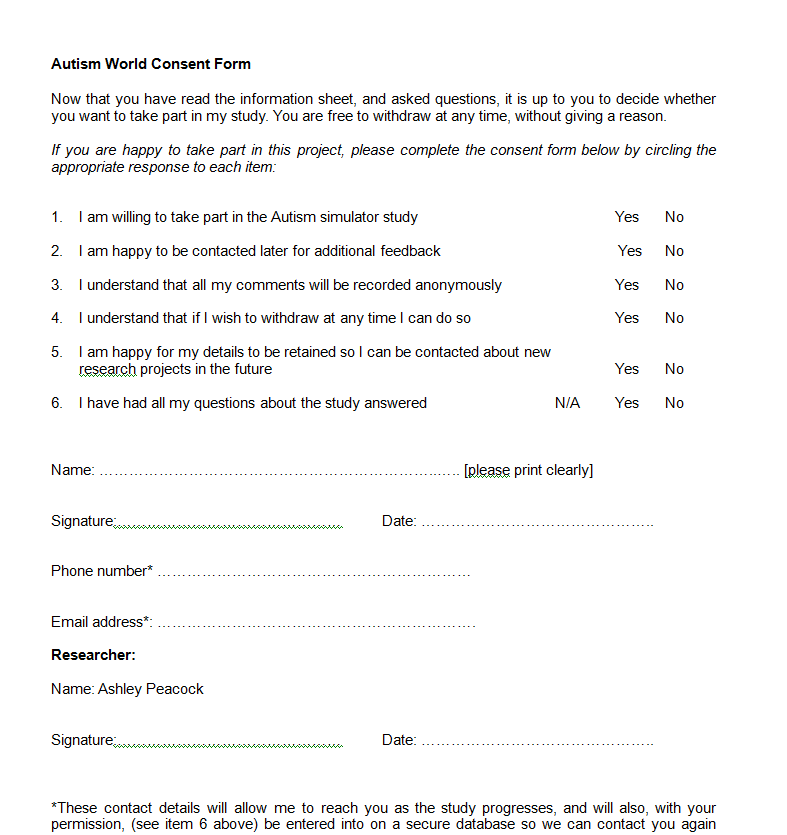
\includegraphics[scale=0.7]{images/appendix/summative_consentform.png}
\caption{Consent form participants were asked to complete}
\end{figure}

\begin{figure}[H]
\centering
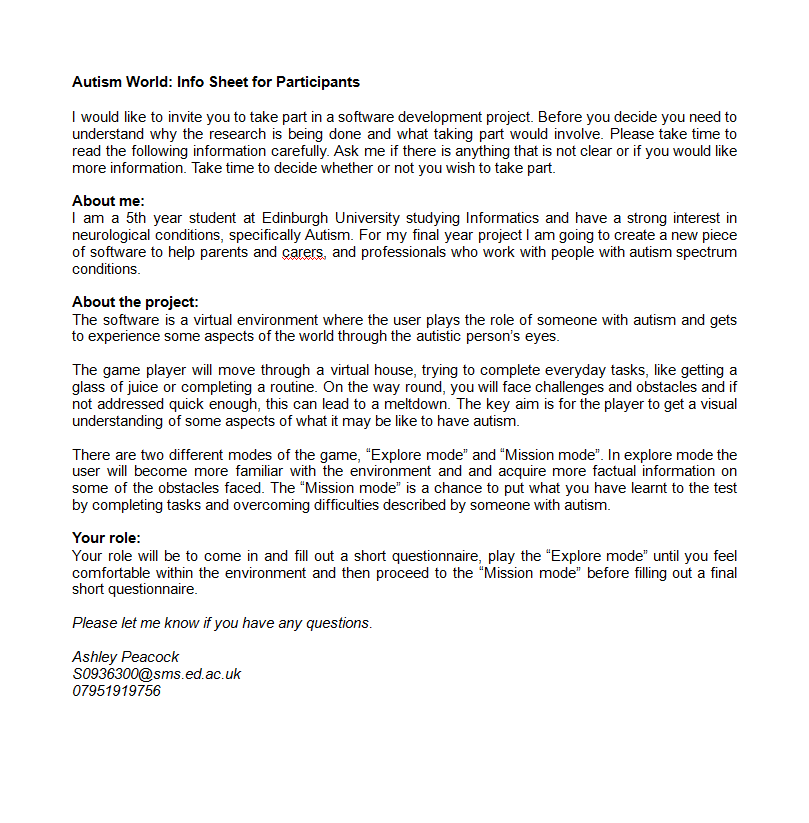
\includegraphics[scale=0.7]{images/appendix/summative_infosheet.png}
\caption{Info sheet partcipants were asked to complete}
\end{figure}

\section{Summative results}
\label{summative_backgroundresults}

\begin{figure}[H]
\centering
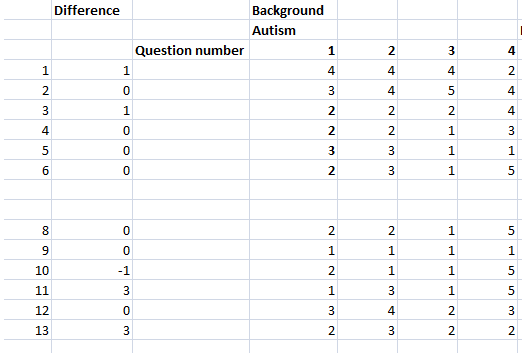
\includegraphics[scale=0.7]{images/appendix/summative_resultsbackground.png}
\caption{Results of background questionnaire and their feelings towards their knowledge with autism. Question numbers indicate the matched questions as in \ref{sum_background}}
\end{figure}

\begin{figure}[H]
\centering
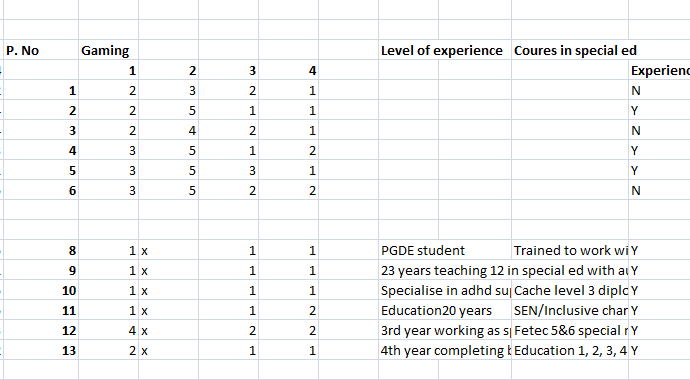
\includegraphics[scale=0.7]{images/appendix/summative_resultsgameexperience.png}
\caption{Shows results of game play experience. The latter give information on background. Y was assigned if they had some experience with autism. N was assigned if they did not. \ref{sum_background}}
\end{figure}

\begin{table}[H]
    \begin{tabular}{| p{1cm} | p{2cm} | p{2cm} | p{3cm} | p{3cm} | p{3cm} |}
    \hline
    \textbf{No} & \textbf{Total before} & \textbf{Total after} & \textbf{Improvement} & \textbf{First Vignette}  \\                                                                                                                                                                                    
	\hline
	1 & 6 & 8 & 2 & A  \\ \hline
	2 & 8 & 8 & 0 & B  \\ \hline
	3 & 6 & 8 & 2 & A  \\ \hline
	4 & 8 & 8 & 0 & B  \\ \hline
	5 & 6 & 6 & 0 & A  \\ \hline
	6 & 8 & 8 & 0 & B \\ \hline
	
	8 & 8 & 8 & 0 & B \\ \hline
	9 & 8 & 8 & 0 & A  \\ \hline
	10 & 6 & 4 & -2 & B  \\ \hline
	11 & 4 & 8 & 4 & A  \\ \hline
	12 & 8 & 8 & 0 & A  \\ \hline
	13 & 4 & 8 & 4 & A  \\ \hline
    \hline
    \end{tabular}
    \caption{Summary of results. Participants 1-6 were in person. Participants 8-12 were online. Participant 13 was in person but completed questionnaire online.}
\end{table}

\section{Summative question responses}
\begin{figure}[H]
\centering
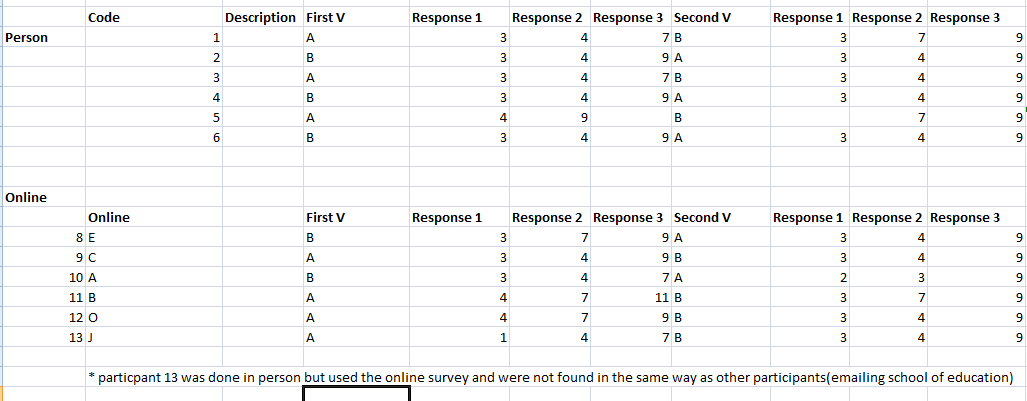
\includegraphics[scale=0.7]{images/appendix/summative_answers.png}
\caption{Individual responses from candidates}
\end{figure}

\begin{figure}[H]
\centering
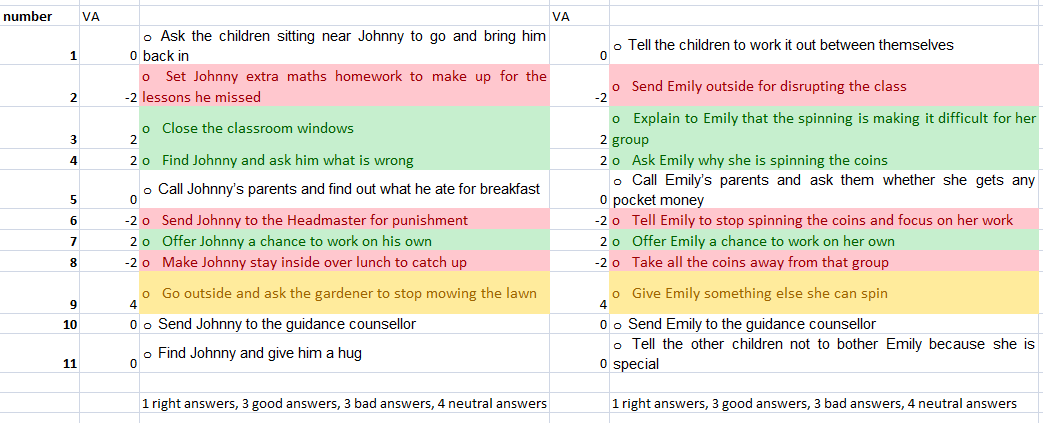
\includegraphics[scale=0.7]{images/appendix/summative_responsescores.png}
\caption{Shows the response numbers and scores assigned}
\end{figure}



\chapter{Prototype implementation}

\section{HouseScene: Code}

\begin{lstlisting}[breaklines=true]

public class HouseScene extends SceneManager {

    public HouseScene(String houseScene, Main app) {
        super(houseScene, app);
    }

    @Override
    public void setupModels() {
        setupLights();
        setupDoors();
        setupDescriptions();

    }
    
    
    public void setupLights() {
        Iterator it = models.keySet().iterator();
        while (it.hasNext()) {
            String key = it.next().toString();
            if(key.contains("lamp")) {
                Spatial node = models.get(key);
                addLampLight(node);
                node.setUserData("state", true);
                node.setUserData("sensory", "lamp");
                System.out.println("Added light to " + key);
                Main.getSensoryManager().addSensoryObject(node, "light");
            }
        }
        
    }
    
    public void setupDescriptions() {
        addDescription("fridge", "This is a fridge and it smells");
        addDescription("fryingpan", "Urg, the smell of this is overpowering");
        addDescription("wardrobe", "Certain clothes can be very uncomfortable for someone with Autism. One person describes"
                + "it as like wearing sand paper, and clothes labels feeling like sandpaper");
        addDescription("tv", "TV Adverts: Parents be warned. If you buy a toy from an advert and it doesn't do"
                + "exactly what the advert says, your child may be quite surprised and upset. Similarly, things on TV "
                + "can be taken very literally and a child with autism may not know they what they see is not real.");
        
    }
    
    public void setupDoors() {
      Iterator it = models.keySet().iterator();
        while (it.hasNext()) {
            String key = it.next().toString();
            if(!key.contains("door")) 
                continue; 
            
            Node door = (Node) models.get(key);
            if(door.getName().contains("door")) {
                DoorControl dc = new DoorControl();
                door.addControl(dc);               
            }
        }
    }

    @Override
    public void setupMaterials() {
        Material m = new Material(am, "Common/MatDefs/Misc/Unshaded.j3md");
        MaterialsManager.addMaterial("unshaded", m); 
    }
}

\end{lstlisting}

\chapter{First version}

\begin{figure}[H]
\centering
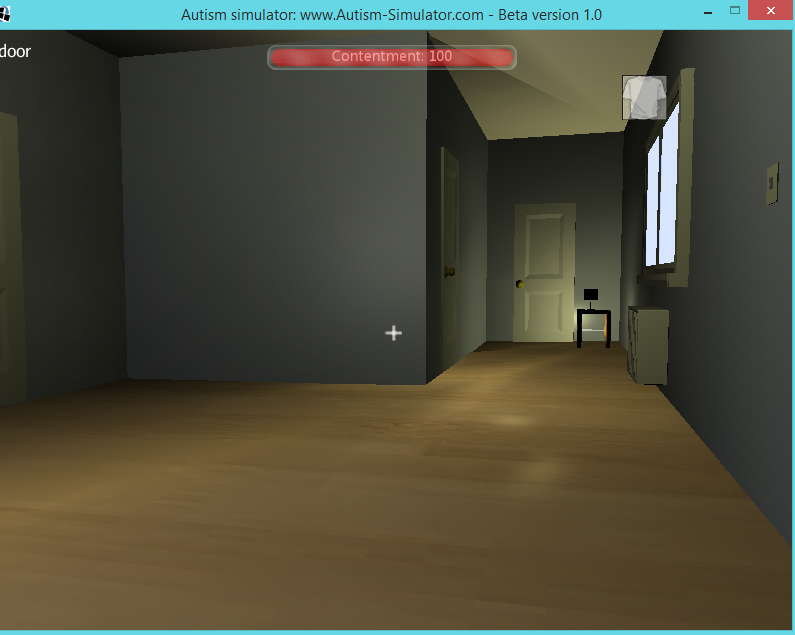
\includegraphics[width=90mm]{images/implementationfirst/gameimages/new_hallway2.png}
\caption{Image of new hallway}
\label{newhallway2}
\end{figure}

\begin{figure}[H]
\centering
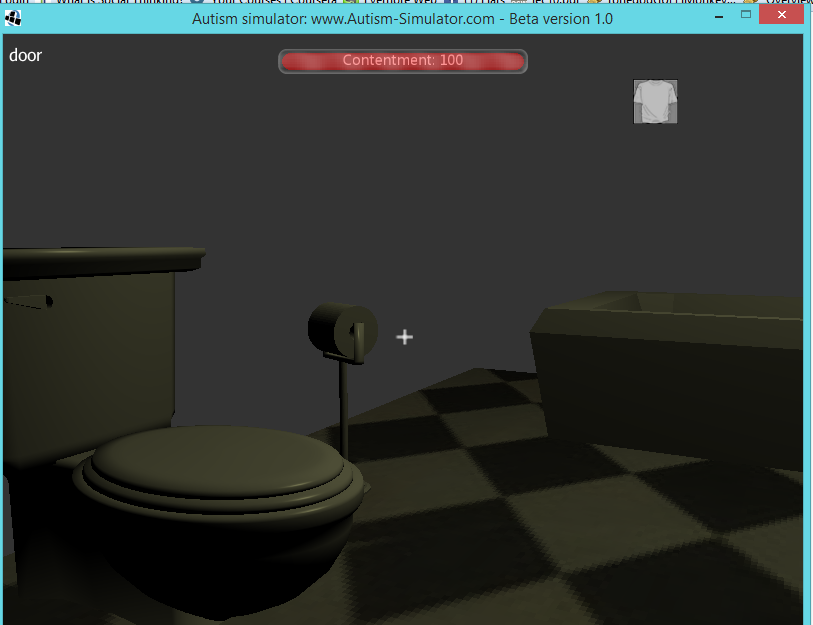
\includegraphics[width=90mm]{images/implementationfirst/gameimages/bathroom1.png}
\caption{Image of bathroom that was previously missing from the house}
\label{old_house}
\end{figure}

\begin{figure}[H]
\centering
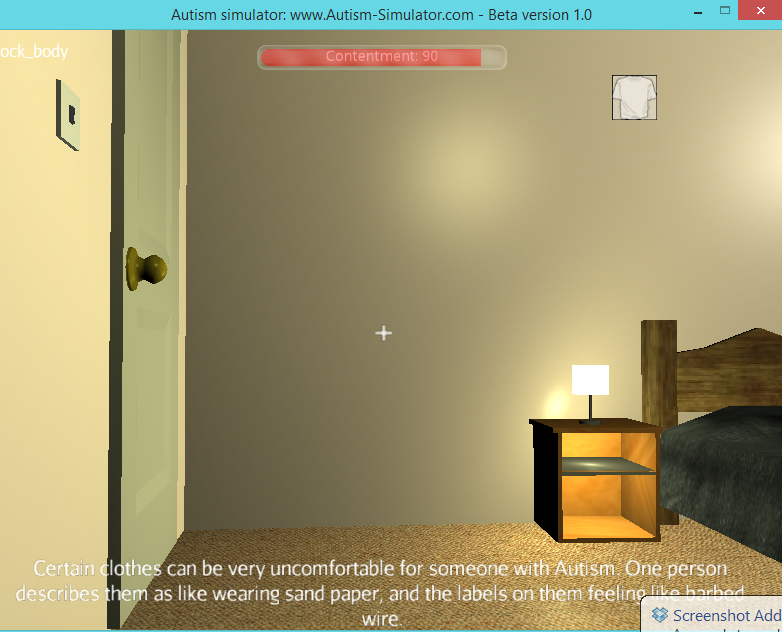
\includegraphics[width=90mm]{images/implementationfirst/gameimages/bedroom_1.png}
\caption{Image of new bedroom}
\label{old_house}
\end{figure}

\begin{figure}[H]
\centering
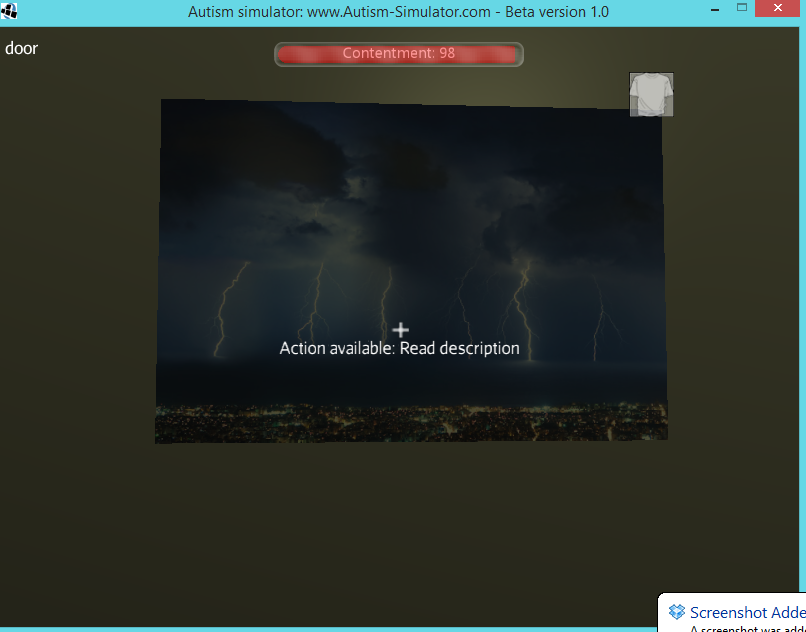
\includegraphics[width=90mm]{images/implementationfirst/gameimages/lighteningposter.png}
\caption{Lightening poster: Gives information in description in regards to autism and unusual fears of lightening}
\label{old_house}
\end{figure}




